\documentclass{standalone}

\usepackage[T1]{fontenc}
\usepackage[utf8]{inputenc}
\usepackage{eulervm}
\usepackage{amsmath}
\usepackage{bm}
\usepackage{tikz}
\usepackage{environ}

\usetikzlibrary{fit}
\usetikzlibrary{patterns}
\usetikzlibrary{arrows}
\usetikzlibrary{automata}

\usepackage{color}

\definecolor{Comment}{RGB}{97,161,176}

\definecolor{btfGreen}{RGB}{51,160,44}
\definecolor{btfRed}{RGB}{190,60,90}

\definecolor{bleuUni}{RGB}{0, 157, 224}
\definecolor{marronUni}{RGB}{68, 58, 49}
\definecolor{grayMarronUni}{RGB}{60, 60, 60}
\definecolor{grayBleuUni}{RGB}{118, 118, 118}

\definecolor{bluecite}{HTML}{009DE0}

\definecolor{Paired-2}{RGB}{166,206,227}
\definecolor{Paired-1}{RGB}{31,120,180}
\definecolor{Paired-4}{RGB}{178,223,138}
\definecolor{Paired-3}{RGB}{51,160,44}
\definecolor{Paired-6}{RGB}{251,154,153}
\definecolor{Paired-5}{RGB}{227,26,28}
\definecolor{Paired-8}{RGB}{253,191,111}
\definecolor{Paired-7}{RGB}{255,127,0}
\definecolor{Paired-10}{RGB}{202,178,214}
\definecolor{Paired-9}{RGB}{106,61,154}
\definecolor{Paired-12}{RGB}{255,255,153}
\definecolor{Paired-11}{RGB}{177,89,40}
\definecolor{Accent-1}{RGB}{127,201,127}
\definecolor{Accent-2}{RGB}{190,174,212}
\definecolor{Accent-3}{RGB}{253,192,134}
\definecolor{Accent-4}{RGB}{255,255,153}
\definecolor{Accent-5}{RGB}{56,108,176}
\definecolor{Accent-6}{RGB}{240,2,127}
\definecolor{Accent-7}{RGB}{191,91,23}
\definecolor{Accent-8}{RGB}{102,102,102}
\definecolor{Spectral-1}{RGB}{158,1,66}
\definecolor{Spectral-2}{RGB}{213,62,79}
\definecolor{Spectral-3}{RGB}{244,109,67}
\definecolor{Spectral-4}{RGB}{253,174,97}
\definecolor{Spectral-5}{RGB}{254,224,139}
\definecolor{Spectral-6}{RGB}{255,255,191}
\definecolor{Spectral-7}{RGB}{230,245,152}
\definecolor{Spectral-8}{RGB}{171,221,164}
\definecolor{Spectral-9}{RGB}{102,194,165}
\definecolor{Spectral-10}{RGB}{50,136,189}
\definecolor{Spectral-11}{RGB}{94,79,162}
\definecolor{Set1-1}{RGB}{228,26,28}
\definecolor{Set1-2}{RGB}{55,126,184}
\definecolor{Set1-3}{RGB}{77,175,74}
\definecolor{Set1-4}{RGB}{152,78,163}
\definecolor{Set1-5}{RGB}{255,127,0}
\definecolor{Set1-6}{RGB}{255,255,51}
\definecolor{Set1-7}{RGB}{166,86,40}
\definecolor{Set1-8}{RGB}{247,129,191}
\definecolor{Set1-9}{RGB}{153,153,153}
\definecolor{Set2-1}{RGB}{102,194,165}
\definecolor{Set2-2}{RGB}{252,141,98}
\definecolor{Set2-3}{RGB}{141,160,203}
\definecolor{Set2-4}{RGB}{231,138,195}
\definecolor{Set2-5}{RGB}{166,216,84}
\definecolor{Set2-6}{RGB}{255,217,47}
\definecolor{Set2-7}{RGB}{229,196,148}
\definecolor{Set2-8}{RGB}{179,179,179}
\definecolor{Dark2-1}{RGB}{27,158,119}
\definecolor{Dark2-2}{RGB}{217,95,2}
\definecolor{Dark2-3}{RGB}{117,112,179}
\definecolor{Dark2-4}{RGB}{231,41,138}
\definecolor{Dark2-5}{RGB}{102,166,30}
\definecolor{Dark2-6}{RGB}{230,171,2}
\definecolor{Dark2-7}{RGB}{166,118,29}
\definecolor{Dark2-8}{RGB}{102,102,102}
\definecolor{Reds-1}{RGB}{255,245,240}
\definecolor{Reds-2}{RGB}{254,224,210}
\definecolor{Reds-3}{RGB}{252,187,161}
\definecolor{Reds-4}{RGB}{252,146,114}
\definecolor{Reds-5}{RGB}{251,106,74}
\definecolor{Reds-6}{RGB}{239,59,44}
\definecolor{Reds-7}{RGB}{203,24,29}
\definecolor{Reds-8}{RGB}{165,15,21}
\definecolor{Reds-9}{RGB}{103,0,13}
\definecolor{Greens-1}{RGB}{247,252,245}
\definecolor{Greens-2}{RGB}{229,245,224}
\definecolor{Greens-3}{RGB}{199,233,192}
\definecolor{Greens-4}{RGB}{161,217,155}
\definecolor{Greens-5}{RGB}{116,196,118}
\definecolor{Greens-6}{RGB}{65,171,93}
\definecolor{Greens-7}{RGB}{35,139,69}
\definecolor{Greens-8}{RGB}{0,109,44}
\definecolor{Greens-9}{RGB}{0,68,27}
\definecolor{Blues-1}{RGB}{247,251,255}
\definecolor{Blues-2}{RGB}{222,235,247}
\definecolor{Blues-3}{RGB}{198,219,239}
\definecolor{Blues-4}{RGB}{158,202,225}
\definecolor{Blues-5}{RGB}{107,174,214}
\definecolor{Blues-6}{RGB}{66,146,198}
\definecolor{Blues-7}{RGB}{33,113,181}
\definecolor{Blues-8}{RGB}{8,81,156}
\definecolor{Blues-9}{RGB}{8,48,107}


\begin{document}
  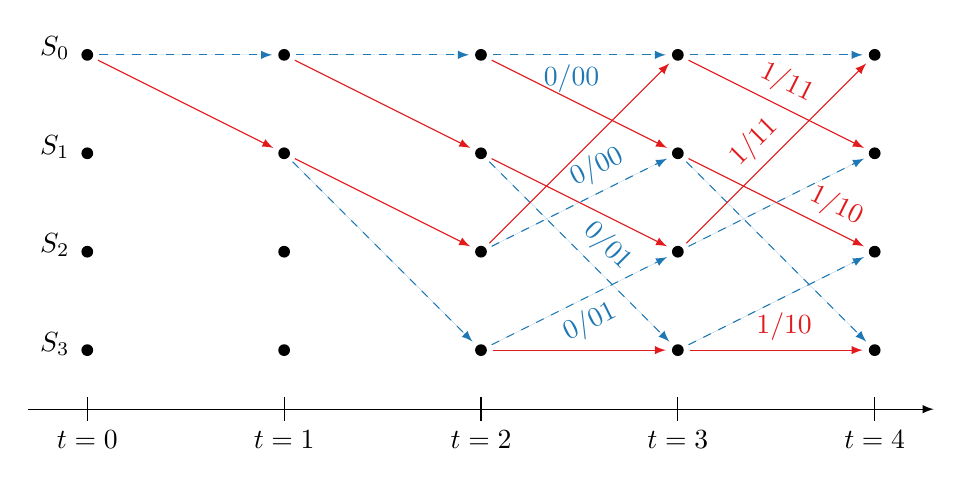
\begin{tikzpicture}%[scale=\tikzscale]
  % \node[state, accepting] (s0) at (+0.0, +0.0) {$S_0$};
  % \node[state           ] (s1) at (-2.0, -1.5) {$S_1$};
  % \node[state           ] (s2) at (+2.0, -1.5) {$S_2$};
  % \node[state           ] (s3) at (-0.0, -3.0) {$S_3$};

  % \tikzset{b0/.style={->,>=latex, draw=Paired-1, shorten >=3pt, shorten <= 3pt, dashed} }
  % \tikzset{b1/.style={->,>=latex, draw=Paired-5, shorten >=3pt, shorten <= 3pt        } }

  % \draw[b1] (s0) to[bend right=30]                (s1) node [midway, above, xshift=-1.5cm, yshift=-0.40cm] {1/11};
  % \draw[b1] (s1) to[bend right=20]                (s2) node [midway, above, xshift=-0.0cm, yshift=-2.50cm] {1/10};
  % \draw[b0] (s1) to[bend right=30]                (s3) node [midway, above, xshift=-1.5cm, yshift=-3.25cm] {0/01};
  % \draw[b0] (s3) to[bend right=30]                (s2) node [midway, above, xshift=+1.5cm, yshift=-3.25cm] {0/01};
  % \draw[b0] (s2) to[bend right=20]                (s1) node [midway, above, xshift=-0.0cm, yshift=-1.10cm] {0/00};
  % \draw[b1] (s2) to[bend right=30]                (s0) node [midway, above, xshift=+1.5cm, yshift=-0.40cm] {1/11};
  % \draw[b1] (s3) to[out=-120,in= -60,looseness=6] (s3) node [midway, above, xshift=+0.0cm, yshift=-4.60cm] {1/10};
  % \draw[b0] (s0) to[out= +60,in=+120,looseness=6] (s0) node [midway, above, xshift=+0.0cm, yshift=+1.00cm] {0/00};


  \newcommand\vsep{2.5}
  \newcommand\hsep{1.25}

  \node (t0_s0) at (0.0,-0.0)               [circle,fill,inner sep=1.5pt, label={[left,xshift=-1mm]$S_0$}]{};
  \node (t0_s1) at (0.0,-\hsep)             [circle,fill,inner sep=1.5pt, label={[left,xshift=-1mm]$S_1$}]{};
  \node (t0_s2) at (0.0,-\hsep-\hsep)       [circle,fill,inner sep=1.5pt, label={[left,xshift=-1mm]$S_2$}]{};
  \node (t0_s3) at (0.0,-\hsep-\hsep-\hsep) [circle,fill,inner sep=1.5pt, label={[left,xshift=-1mm]$S_3$}]{};

  \node (t1_s0) at (\vsep,-0.0)               [circle,fill,inner sep=1.5pt]{};
  \node (t1_s1) at (\vsep,-\hsep)             [circle,fill,inner sep=1.5pt]{};
  \node (t1_s2) at (\vsep,-\hsep-\hsep)       [circle,fill,inner sep=1.5pt]{};
  \node (t1_s3) at (\vsep,-\hsep-\hsep-\hsep) [circle,fill,inner sep=1.5pt]{};

  \node (t2_s0) at (\vsep+\vsep,-0.0)               [circle,fill,inner sep=1.5pt]{};
  \node (t2_s1) at (\vsep+\vsep,-\hsep)             [circle,fill,inner sep=1.5pt]{};
  \node (t2_s2) at (\vsep+\vsep,-\hsep-\hsep)       [circle,fill,inner sep=1.5pt]{};
  \node (t2_s3) at (\vsep+\vsep,-\hsep-\hsep-\hsep) [circle,fill,inner sep=1.5pt]{};

  \node (t3_s0) at (\vsep+\vsep+\vsep,-0.0)               [circle,fill,inner sep=1.5pt]{};
  \node (t3_s1) at (\vsep+\vsep+\vsep,-\hsep)             [circle,fill,inner sep=1.5pt]{};
  \node (t3_s2) at (\vsep+\vsep+\vsep,-\hsep-\hsep)       [circle,fill,inner sep=1.5pt]{};
  \node (t3_s3) at (\vsep+\vsep+\vsep,-\hsep-\hsep-\hsep) [circle,fill,inner sep=1.5pt]{};

  \node (t4_s0) at (\vsep+\vsep+\vsep+\vsep,-0.0)               [circle,fill,inner sep=1.5pt]{};
  \node (t4_s1) at (\vsep+\vsep+\vsep+\vsep,-\hsep)             [circle,fill,inner sep=1.5pt]{};
  \node (t4_s2) at (\vsep+\vsep+\vsep+\vsep,-\hsep-\hsep)       [circle,fill,inner sep=1.5pt]{};
  \node (t4_s3) at (\vsep+\vsep+\vsep+\vsep,-\hsep-\hsep-\hsep) [circle,fill,inner sep=1.5pt]{};

  \draw[->,>=latex] (-0.75,-\hsep-\hsep-\hsep-0.75) -- (\vsep+\vsep+\vsep+\vsep+0.75,-\hsep-\hsep-\hsep-0.75);

  \draw[- ,>=latex] (0.0,                    -\hsep-\hsep-\hsep-0.6) -- (0.0,                    -\hsep-\hsep-\hsep-0.9) node [below, xshift=+0.0cm, yshift=+0.00cm] {$t = 0$};
  \draw[- ,>=latex] (\vsep,                  -\hsep-\hsep-\hsep-0.6) -- (\vsep,                  -\hsep-\hsep-\hsep-0.9) node [below, xshift=+0.0cm, yshift=+0.00cm] {$t = 1$};
  \draw[- ,>=latex] (\vsep+\vsep,            -\hsep-\hsep-\hsep-0.6) -- (\vsep+\vsep,            -\hsep-\hsep-\hsep-0.9) node [below, xshift=+0.0cm, yshift=+0.00cm] {$t = 2$};
  \draw[- ,>=latex] (\vsep+\vsep+\vsep,      -\hsep-\hsep-\hsep-0.6) -- (\vsep+\vsep+\vsep,      -\hsep-\hsep-\hsep-0.9) node [below, xshift=+0.0cm, yshift=+0.00cm] {$t = 3$};
  \draw[- ,>=latex] (\vsep+\vsep+\vsep+\vsep,-\hsep-\hsep-\hsep-0.6) -- (\vsep+\vsep+\vsep+\vsep,-\hsep-\hsep-\hsep-0.9) node [below, xshift=+0.0cm, yshift=+0.00cm] {$t = 4$};

  \tikzset{b0/.style={->,>=latex, draw=Paired-1, fill=Paired-1, shorten >=2pt, shorten <= 2pt, dashed} }
  \tikzset{b1/.style={->,>=latex, draw=Paired-5, fill=Paired-5, shorten >=2pt, shorten <= 2pt        } }

  \draw[b0] (t0_s0) -- (t1_s0); % node [midway, above, sloped, text=Paired-1] {0/00};
  \draw[b1] (t0_s0) -- (t1_s1); % node [midway, above, sloped, text=Paired-5] {1/11};

  \draw[b0] (t1_s0) -- (t2_s0); % node [midway, above, sloped, text=Paired-1] {0/00};
  \draw[b1] (t1_s0) -- (t2_s1); % node [midway, above, sloped, text=Paired-5] {1/11};
  \draw[b0] (t1_s1) -- (t2_s3); % node [midway, above, sloped, text=Paired-1] {0/01};
  \draw[b1] (t1_s1) -- (t2_s2); % node [midway, above, sloped, text=Paired-5] {1/10};


  \draw[b0] (t2_s0) -- (t3_s0) node [midway, below, text=Paired-1, sloped, xshift=-1mm,] {0/00};
  \draw[b1] (t2_s0) -- (t3_s1); % node [midway, above, text=Paired-5] {};
  \draw[b0] (t2_s1) -- (t3_s3) node [midway, above, text=Paired-1, sloped, xshift=+2mm] {0/01};
  \draw[b1] (t2_s1) -- (t3_s2); % node [midway, above, text=Paired-5] {};
  \draw[b0] (t2_s2) -- (t3_s1) node [midway, above, text=Paired-1, sloped, xshift=+4mm] {0/00};
  \draw[b1] (t2_s2) -- (t3_s0); % node [midway, above, text=Paired-5] {};
  \draw[b0] (t2_s3) -- (t3_s2) node [midway, below, text=Paired-1, sloped, xshift=+0mm] {0/01};
  \draw[b1] (t2_s3) -- (t3_s3); % node [midway, above, text=Paired-5] {};

  \draw[b0] (t3_s0) -- (t4_s0); % node [midway, above, text=Paired-1] {};
  \draw[b1] (t3_s0) -- (t4_s1) node [midway, above, text=Paired-5, sloped, xshift=-0mm] {1/11};
  \draw[b0] (t3_s1) -- (t4_s3); % node [midway, above, text=Paired-1] {};
  \draw[b1] (t3_s1) -- (t4_s2) node [midway, above, text=Paired-5, sloped, xshift=+7mm] {1/10};
  \draw[b0] (t3_s2) -- (t4_s1); % node [midway, above, text=Paired-1] {};
  \draw[b1] (t3_s2) -- (t4_s0) node [midway, above, text=Paired-5, sloped, xshift=-1mm] {1/11};
  \draw[b0] (t3_s3) -- (t4_s2); % node [midway, above, text=Paired-1] {};
  \draw[b1] (t3_s3) -- (t4_s3) node [midway, above, text=Paired-5, sloped, xshift=+1mm] {1/10};

  \end{tikzpicture}
\end{document}